%%%%%%%%%%%%%%%%%%%%%%%%%%%%%%%%%%%%%%%%%%%%%%%%%%%%%%%%%%%%%%%%%%%%%%%%%%%%%%%%%%%
\section{Aim}
\label{sec:4aim}
%%%%%%%%%%%%%%%%%%%%%%%%%%%%%%%%%%%%%%%%%%%%%%%%%%%%%%%%%%%%%%%%%%%%%%%%%%%%%%%%%%%

Develop an understanding of methods to evaluate predictions of exposure from hybrid models

%%%%%%%%%%%%%%%%%%%%%%%%%%%%%%%%%%%%%%%%%%%%%%%%%%%%%%%%%%%%%%%%%%%%%%%%%%%%%%%%%%%
\section{Objectives}
\label{sec:4objectives}
%%%%%%%%%%%%%%%%%%%%%%%%%%%%%%%%%%%%%%%%%%%%%%%%%%%%%%%%%%%%%%%%%%%%%%%%%%%%%%%%%%%

\begin{itemize}
    \item Establish how to use mobile monitoring equipment to replicate static monitoring site datasets (which are used for air quality model evaluation)
    \item Collect mobile monitoring data representative of a journey from the LHEM
    \item Model exposure of this journey using LHEM methodology
    \item Compare the monitored and modelled exposures
\end{itemize}

%%%%%%%%%%%%%%%%%%%%%%%%%%%%%%%%%%%%%%%%%%%%%%%%%%%%%%%%%%%%%%%%%%%%%%%%%%%%%%%%%%%
\section{Background}
\label{sec:4background}
%%%%%%%%%%%%%%%%%%%%%%%%%%%%%%%%%%%%%%%%%%%%%%%%%%%%%%%%%%%%%%%%%%%%%%%%%%%%%%%%%%%

The focus of this PhD research so far has been on developing a dynamic exposure model to better understand exposure to urban air pollution in the population of London. Having reconstructed the time-activity of the population, their exposure to PM$_{2.5}$ and NO$_{2}$ was modelled, and then refined, with further investigation of the London Underground micro-environment. This next chapter will consider how to evaluate the NO$_{2}$ results that are calculated using an exposure model of this style.

I defined the features that a hybrid exposure model should have in Section \ref{sec:dynamic_hybrid_models} as \textit{"It should have highly temporal and spatially resolved air quality inputs which consider both indoor and outdoor sources (including regional and local source for the latter), it should be able to model infiltration rates for different modes of transport and building types, it should reflect the multiple micro-environments that people spend their time in (and take account of the temporal resolution of these) and finally it should (for linkage through to epidemiological end-points) be able to consider different breathing rates to quantify exposure and dose for multiple pollutants"}. Section \ref{sec:dynamic_hybrid_models} examined models that were within this wider field (of varying levels of complexity), but it was noticeable that there was little evaluation of the exposure predictions that they made. There are to my knowledge no established protocols for evaluating exposure predictions from a hybrid/dynamic exposure model, as this type of method and field of research is relatively new. In addition, as the field grows the exact approaches are being refined and vary between studies, meaning one evaluation method would unlikely be fit for the next study. Possible sources of error in this type of model are classified in Table \ref{tab:exposure_error_table}, with a brief description, and whether they are unique to exposure models of this kind.

\newgeometry{margin=0.7cm}
\thispagestyle{empty}
\begin{landscape}

\begin{table}[]
\centering
\begin{tabular}{ | p{3cm} | p{13.2cm} | p{7.7cm} |}
\hline
\textbf{Type of uncertainty/error} & \textbf{Description} & \textbf{Hybrid specific} \\ \hline
        Air quality annual average monitoring site predictions  &  Evaluation exercises of air quality models using high quality monitoring site data demonstrate that they (in our case CMAQ-UK) can make predictions of annual averages of most pollutants with reasonable accuracy.         &  No, CMAQ-UK and other similar models are commonly used in static exposure studies.         \\ \hline
        
        Air quality annual average non-monitoring site predictions  &  How air quality models predict concentrations in locations that are not readily available for evaluation via monitoring sites is not well understood.         &   No, CMAQ-UK and other similar models are commonly used in static exposure studies.        \\ \hline
        
        Air quality temporal resolution  &  Annual averages are often used for exposure studies, which are relatively easy to quantify against monitoring sites (see above). However the complexity of the hybrid model we are now considering uses hourly diurnal profiles, which vary in their accuracy of prediction over time, and therefore the accuracy of their input to exposure varies by time of the day, and day of the week.         &   Partly. Not many static studies of large groups of people consider exposure at high temporal resolution (because they normally use annual averages), and even less quantify and include the errors that this produces.        \\ \hline
        
        Micro-environmental modelling  &   Mass-balance models and I/O ratios to estimate the concentrations of pollutants within microenvironments, in relation to outdoor concentrations, are inherently subject to variation due to the inexact inputs. Literature reviews to establish ‘best-guess’ I/O ratios are common but their transfer-ability to other counties/cities is often unknown. Monte-Carlo simulation of the inputs to create a range of predictions can be undertaken to understand their impact.         &    Yes. Static exposure studies normally use outdoor concentrations for exposure assessment. Exposure assessments of the health effects of environments i.e. indoor, may use micro-environmental modelling and I/O ratios, but not in conjunction with people’s movements, multiple environments, and high spatial-temporal air quality.       \\ \hline
        
        Temporal representative errors of exposure  &   Exposure predictions for a person over a time period can be made, but the degree to which these predictions are representative of that person’s exposure for that period of time are unknown. In the LHEM the exposures were calculated based on the person’s previous days’ movements, and the respondents were asked whether this was representative of their typical day; but quantifying the difference between the day of the data collected and their ‘typical’ day in terms of exposure is not explored.         &    Yes. Hybrid exposure studies that consider the exposure of individuals through space-time, especially those that seek to frame exposure results in terms of longer-term health effects, need to develop methods to estimate the variability of representativeness error.       \\ \hline
        
        Representative errors of groups and populations  &   Extrapolating exposure predictions from a small group of people (e.g. a classroom of 30 ten year olds in South London), to larger groups of people (e.g. all school children in London) can be controlled in part by statistical sampling techniques and appropriate power calculations. But this can only be done with prior data/knowledge of the population, which while fairly simple to do for basic demographics using Census data and similar, is much more difficult to do for exposure prediction models. To ensure representativeness exposure sample calculations need to ensure that important drivers of exposure i.e. tube usage, are included alongside more standard variables.        &   No, other exposure methods have this issue, but it is often not addressed fully. Studies with larger numbers of participants would be expected to have a better range of exposures and be more representative.        \\ \hline
\end{tabular}
\caption{Errors and uncertainty in exposure models}
\label{tab:exposure_error_table}
\end{table}

\end{landscape}

\restoregeometry

The next sections of the background to this chapter are discussed around the types of uncertainty from Table \ref{tab:exposure_error_table} above.

%%%%%%%%%%%%%%%%%%%%%%%%%%%%%%
\subsection{Air quality annual average monitoring site predictions}
\label{air_quality_annual_average_predictions}
%%%%%%%%%%%%%%%%%%%%%%%%%%%%%%

Air quality models used in hybrid exposure studies are often evaluated against annual averages from monitoring sites in the cities of the study. For example \cite{DeNazelle2013} study in Barcelona used a dispersion model (\cite{Lao2011}) for the NO$_{2}$ air quality inputs to their exposure model, and showed good performance/agreement (Table \ref{tab:fig:de_nazelle_model_performance}) with errors in the range of -12\% to +10\%.

\begin{figure}[H]
\centering
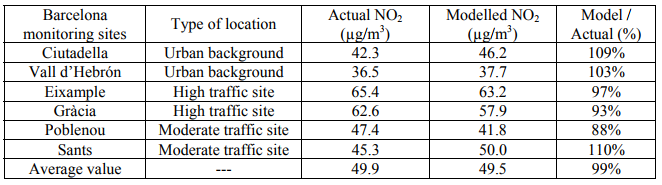
\includegraphics[scale=1.4]{de_nazelle_model_performance}
\caption{Performance statistics of an air quality model used in \cite{DeNazelle2013}}
\label{tab:fig:de_nazelle_model_performance}
\end{figure}

By understanding the scale of these errors in the air quality model, if it is presumed that they are uniform in time and space across the study area (discussed more below), then they can be incorporated into a static exposure study of outdoor air at household addresses or similar.

%%%%%%%%%%%%%%%%%%%%%%%%%%%%%%
\subsection{Air quality annual average non-monitoring site predictions}
\label{air_quality_annual_average_non_site_predictions}
%%%%%%%%%%%%%%%%%%%%%%%%%%%%%%

The predictions of air quality models, away from monitoring sites, is less well understood. Taking our 2016 CMAQ-UK model the NO$_{2}$ map of London shown in Figure \ref{fig:cmaq_and_monitoring_sites} (below) illustrates the location of monitoring sites i.e. where the predictions have been evaluated and understood. Clearly there are many areas which are not evaluated; there are 16 million cells in the raster, and only 242 sites (many of which are either not operational, do not have a high enough data capture rate for comparison, or do not measure the pollutants we are interested in, meaning the actual number is far less). This means that only ~0.0015\% of the locations shown in Figure \ref{fig:cmaq_and_monitoring_sites} have been evaluated and the possible error (between model prediction and measurement) understood.

\begin{figure}[H]
\centering
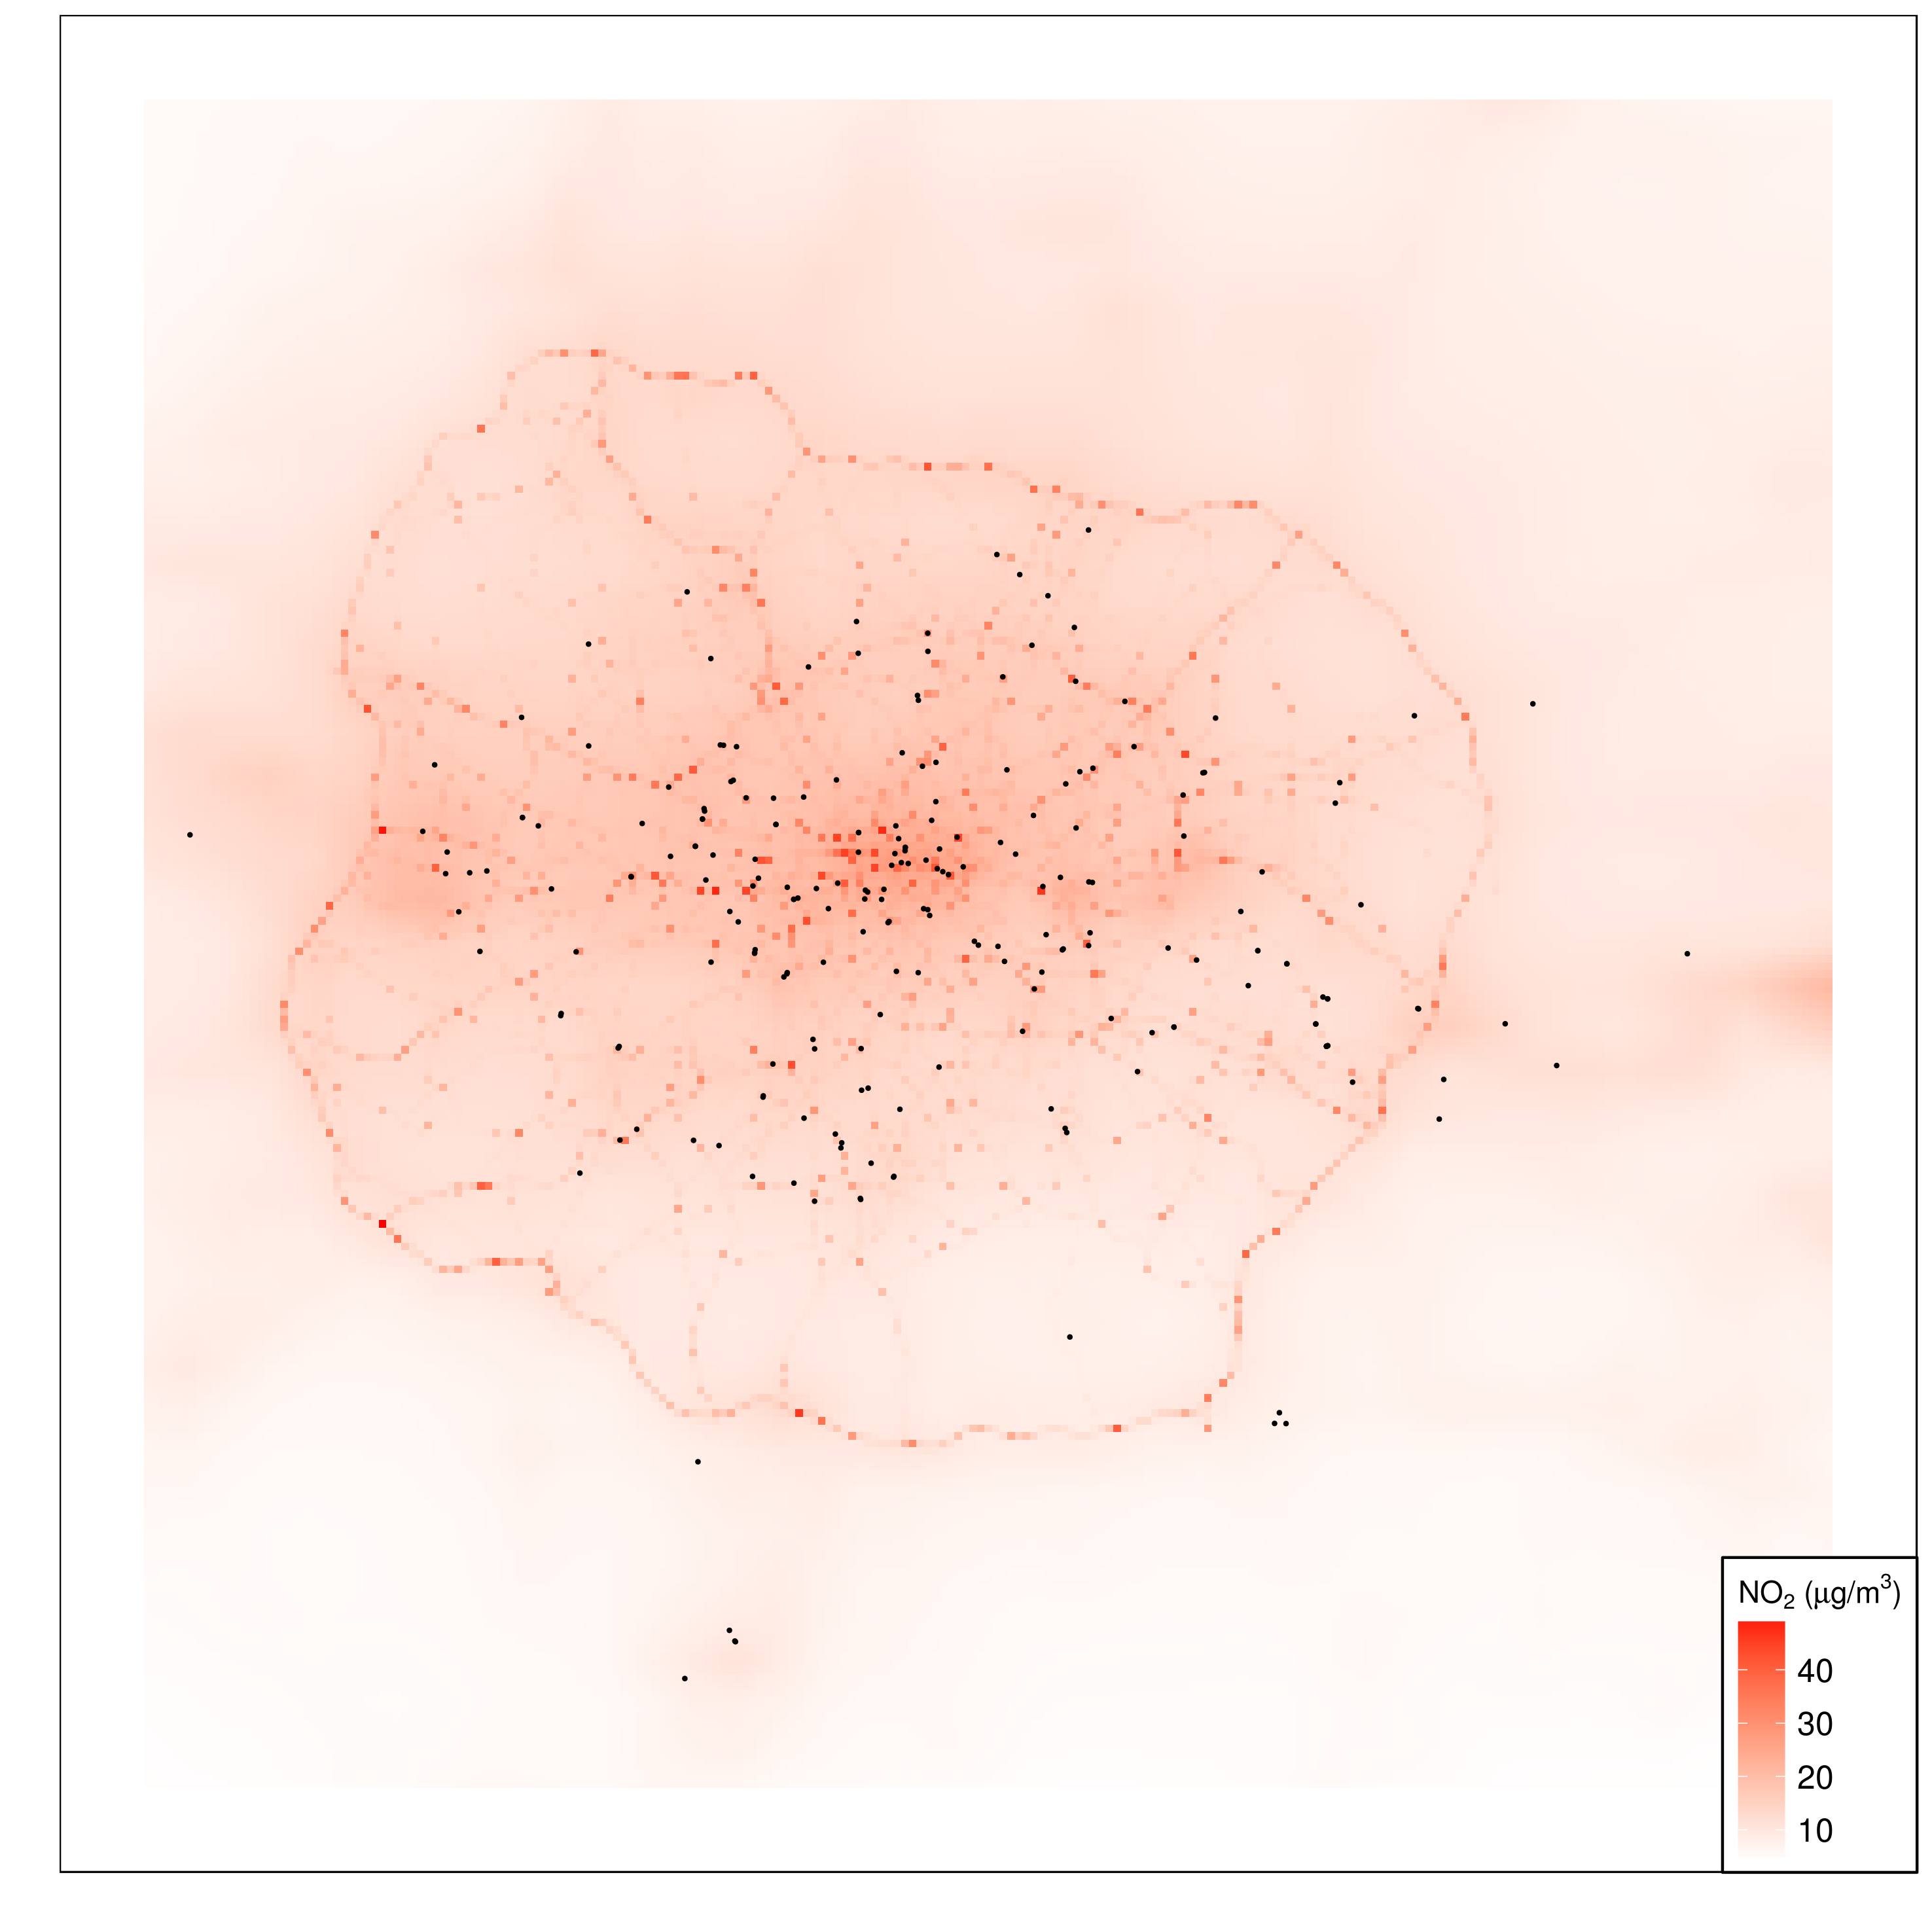
\includegraphics[scale=0.5]{images/cmaq_and_monitoring_sites.png}
\caption{CMAQ-UK for London + Air Quality monitoring sites}
\label{fig:cmaq_and_monitoring_sites}
\end{figure}

For these non-monitoring site locations, we presume that the model functions in the same manner, with the same error levels. In reality it seems likely that there are varying degrees of accuracy. This may be less of a concern within an exposure model looking at health effects between areas of high/low concentrations, providing it represents the spatial pattern adequately i.e. predicting lower concentrations and higher concentrations in the right places, even if the concentrations themselves are not exactly right. As part of this chapter I am going to aim to better understand how the model predicts away from monitoring sites. It is impractical to place a monitoring site at every location, so I will develop a method whereby I use mobile monitoring devices in-lieu of monitoring sites. As background to this, I searched for studies which have already attempted this. There is a small amount of literature which has tried to evaluate air quality away from monitoring sites using mobile monitors. \cite{Buteau2017} compared a number of methods for predicting concentrations of O3 and NO$_{2}$ in Montreal, Canada at the level three-character postal code area (~6km$^{2}$ square). Alongside traditional spatial interpolation using inverse-distance weighting, and nearest monitoring site methods, they also based a land-use regression model upon a dense monitoring survey. However, these were semi-permanent monitors at fixed sites for 9 months of a year, and so whilst their results were encouraging the method is not really transferable to portable monitors that I intend to use. \cite{Shi2016} also created a land-use regression model, with mobile measurements as an input, which achieved good results, but their study was based on repeated measurements using vehicles sampling along a set route for 14 consecutive days, and the choice of 14 rather than say 20 seemed to be a function of their available sampling time rather than calculated using statistical analysis.

%%%%%%%%%%%%%%%%%%%%%%%%%%%%%%
\subsection{Air quality temporal predictions}
\label{air_quality_temporal_predictions}
%%%%%%%%%%%%%%%%%%%%%%%%%%%%%%

Air quality models that use a higher temporal resolution have more sources of error to quantify and include in an exposure model than one which uses annual averages. As an annual average value, a difference of +/- 5 $\mu \text{g m}^{-3}$ between the model and the measurements can be factored into the exposure prediction relatively easily. But if the model is predicting a concentration every hour then this error will vary for each hour i.e. 8760 hours resulting in 8760 model/measurement differences.

%%%%%%%%%%%%%%%%%%%%%%%%%%%%%%
\subsection{Micro-environmental modelling}
\label{microenvironmental_modelling}
%%%%%%%%%%%%%%%%%%%%%%%%%%%%%%

Within dynamic exposure models, exposure in microenvironments is often calculated in relation to outdoor concentrations. Therefore, in addition to the uncertainty of the air quality predictions in a place and time, further uncertainty is added when the outdoor concentration is ‘converted’ to a microenvironment concentration (whether this is done using an I/O ratio for indoor concentrations, or a mass-balance model as used in Section \ref{sec:in_vehicle_modelling}). Exposures in the LHEM, for all environments except the London Underground, used the CMAQ-UK air quality model as an input. \cite{Dhondt2012} described the possible sources of error within the in-vehicle section of their dynamic model, and noted that the air quality inputs may not be of a high enough spatial resolution to capture concentration gradients near roads adequately. But they did not seek to evaluate the individual-level daily/weekly/hourly concentrations, and indeed due to the type of the study (an aggregated population) they would have found it difficult to do so (due to the large numbers of individuals). Similarly and whilst this was evaluated at monitoring sites (Figure \ref{tab:fig:de_nazelle_model_performance}), no monitoring attempt at individual level exposure evaluation was undertaken.

%%%%%%%%%%%%%%%%%%%%%%%%%%%%%%
\subsection{Representative errors}
\label{representative_errors}
%%%%%%%%%%%%%%%%%%%%%%%%%%%%%%

Exposure predictions for an individual or group, over a time period, can be made using dynamic models. But the degree to which these predictions are representative of that exposure for that period of time is a source of uncertainty. Similarly, the degree to which predicting exposure for a group or groups of people, and extrapolating to the wider population, is a further source of confusion and error. In the LHEM, the exposures for each individual were calculated based on the person’s previous days’ movements, and they were asked whether this was representative of their typical day. Analysing the responses to the latter question showed us that most of the subjects had a fairly set pattern of movement (and therefore likely exposure), but the degree of the variance between their typical day and a non-typical day is unknown, and indeed how many ‘non-typical days’ do they have? One way to evaluate the exposure predictions from our model would have been to distribute personal monitors to all the LTDS participants, for an entire year, collect and process the data, and then compare it to the LHEM predictions to see whether our ‘snap shot’ day exposure was close to their annual average day exposure. However, there were ~45,000 subjects, meaning a huge number of personal monitors and logistical support would have been needed, and it was therefore unfeasible. A method to make this more manageable might be to develop a statistical model whereby an appropriate sample-size is calculated. That is, just sampling a percentage of the 45,000, but in the knowledge that they will have a similar distribution of exposures to the total population of the study; then giving this smaller subset of participants monitors for a prolonged period of time and understanding the daily changes in their exposure. This is explored more in Methods (Section \ref{sec:4methods}) 

%%%%%%%%%%%%%%%%%%%%%%%%%%%%%%%%%%%%%%%%%%%%%%%%%%%%%%%%%%%%%%%%%%%%%%%%%%%%%%%%%%%
\section{Methods}
\label{sec:4methods}
%%%%%%%%%%%%%%%%%%%%%%%%%%%%%%%%%%%%%%%%%%%%%%%%%%%%%%%%%%%%%%%%%%%%%%%%%%%%%%%%%%%

We can now see that there are a number of difficult and challenging sources of error to consider in evaluating a hybrid exposure model. Air quality models have quantifiable errors in their predictions at the monitoring sites they are evaluated against, errors at locations away from monitoring sites which are not well understood, further variation and errors when using a high time resolution air quality model, errors in the micro-environmental modelling, and more errors in terms of the representativeness of the exposure predictions arrived at. The following methods section outlines how I attempt to mitigate some of these sources of error, remove some of the others, and produce an evaluation of one short journey; comparing the LHEM prediction of this journey to measured exposure using personal monitoring. The process is summarised below in Figure X.

\begin{figure}[H]
\centering
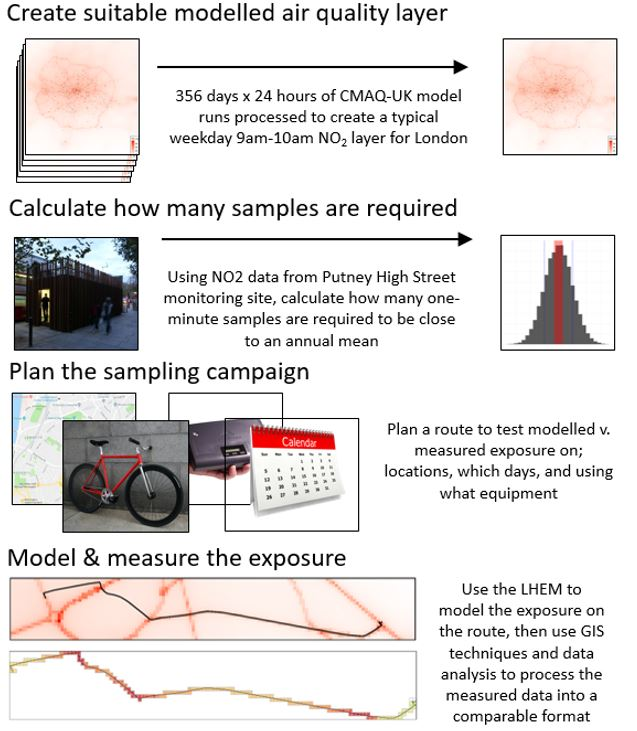
\includegraphics[scale=0.8]{images/comparison_method_summary.jpg}
\caption{Method summary}
\label{fig:comparison_method_summary}
\end{figure}

%%%%%%%%%%%%%%%%%%%%%%%%%%%%%%
\subsection{Estimating repeat journey numbers}
\label{evaluation_journey_numbers}
%%%%%%%%%%%%%%%%%%%%%%%%%%%%%%


%%%%%%%%%%%%%%%%%%%%%%%%%%%%%%%%%%%%%%%%%%%%%%%%%%%%%%%%%%%%%%%%%%%%%%%%%%%%%%%%%%%
\section{Results}
\label{sec:4results}
%%%%%%%%%%%%%%%%%%%%%%%%%%%%%%%%%%%%%%%%%%%%%%%%%%%%%%%%%%%%%%%%%%%%%%%%%%%%%%%%%%%


%%%%%%%%%%%%%%%%%%%%%%%%%%%%%%%%%%%%%%%%%%%%%%%%%%%%%%%%%%%%%%%%%%%%%%%%%%%%%%%%%%%
\section{Discussion}
\label{sec:4Discussion}
%%%%%%%%%%%%%%%%%%%%%%%%%%%%%%%%%%%%%%%%%%%%%%%%%%%%%%%%%%%%%%%%%%%%%%%%%%%%%%%%%%%


%%%%%%%%%%%%%%%%%%%%%%%%%%%%%%%%%%%%%%%%%%%%%%%%%%%%%%%%%%%%%%%%%%%%%%%%%%%%%%%%%%%
\section{Conclusions}
\label{sec:4conclusions}
%%%%%%%%%%%%%%%%%%%%%%%%%%%%%%%%%%%%%%%%%%%%%%%%%%%%%%%%%%%%%%%%%%%%%%%%%%%%%%%%%%%